\documentclass[11pt,a4paper]{article}
\usepackage[utf8]{inputenc}
\usepackage[T1]{fontenc}
\usepackage{graphicx}
\usepackage{booktabs}
\usepackage{hyperref}
\usepackage{xcolor}
\usepackage{listings}
\usepackage{geometry}
\usepackage{float}
\usepackage{subcaption}

\geometry{margin=1in}

\definecolor{codegreen}{rgb}{0,0.6,0}
\definecolor{codegray}{rgb}{0.5,0.5,0.5}
\definecolor{codepurple}{rgb}{0.58,0,0.82}
\definecolor{backcolour}{rgb}{0.95,0.95,0.92}

\lstdefinestyle{mystyle}{
    backgroundcolor=\color{backcolour},
    commentstyle=\color{codegreen},
    keywordstyle=\color{magenta},
    numberstyle=\tiny\color{codegray},
    stringstyle=\color{codepurple},
    basicstyle=\ttfamily\footnotesize,
    breakatwhitespace=false,
    breaklines=true,
    captionpos=b,
    keepspaces=true,
    numbers=left,
    numbersep=5pt,
    showspaces=false,
    showstringspaces=false,
    showtabs=false,
    tabsize=2
}
\lstset{style=mystyle}

\title{\textbf{Litespark-Inf: High-Performance SIMD Kernels for BitNet CPU Inference}}
\author{Mindbeam AI}
\date{February 2026}

\begin{document}

\maketitle

\begin{abstract}
We present Litespark-Inf, a high-performance CPU inference library for BitNet ternary neural networks. Our custom SIMD kernels exploit the ternary weight structure $\{-1, 0, +1\}$ to eliminate floating-point multiplication entirely, replacing it with integer addition and subtraction via hardware dot product instructions. We provide optimized implementations for three major CPU architectures: AVX-512 VNNI (Intel Ice Lake+, AMD Zen4+), AVX-VNNI (Intel Core Ultra), and NEON SDOT (Apple Silicon M1--M4). Benchmarks demonstrate \textbf{1.02--1.57$\times$ speedup} over MS BitNet on x86 platforms, with throughput reaching \textbf{11.2 tokens/s} on AVX-512 and \textbf{9.08 tokens/s} on Apple M4.
\end{abstract}

\section{Introduction}

BitNet b1.58, Microsoft's ternary neural network architecture, constrains all weights to $\{-1, 0, +1\}$, theoretically eliminating the need for multiplication in matrix operations. However, existing implementations do not fully exploit this structure.

Litespark-Inf addresses this gap with custom SIMD kernels that:
\begin{itemize}
    \item Replace matrix multiplication with conditional addition/subtraction
    \item Leverage hardware integer dot product instructions (VPDPBUSD, SDOT)
    \item Achieve 14$\times$ memory reduction (556 MB vs 8 GB for float32)
    \item Provide automatic platform detection and kernel selection
\end{itemize}

\section{Usage}

\subsection{Installation}

\begin{lstlisting}[language=bash]
pip install litespark-inf
\end{lstlisting}

\subsection{Python API}

\begin{lstlisting}[language=Python]
from litespark_inf import load_model

model, tokenizer = load_model("bitnet-2b")
input_ids = tokenizer.encode("Hello, world!", return_tensors="pt")
output = model.generate(input_ids, max_new_tokens=100)
print(tokenizer.decode(output[0]))
\end{lstlisting}

\subsection{Command-Line Interface}

\begin{lstlisting}[language=bash]
litespark-inf generate "The meaning of life is"
litespark-inf chat
litespark-inf benchmark
\end{lstlisting}

\subsection{Configuration Options}

The kernel uses optimized tiling parameters configured in the C++ source:

\begin{lstlisting}[language=C++]
// matmul_free_tmac_vnni.cpp
constexpr int TILE_M = 4;    // Rows per tile
constexpr int TILE_N = 64;   // Columns per tile
constexpr int TILE_K = 256;  // Inner dimension per tile
\end{lstlisting}

Thread count is configurable at runtime via the \texttt{num\_threads} parameter.

\section{Optimizations}

\subsection{SIMD Kernel Implementation}

Our kernels exploit the ternary weight structure to eliminate multiplication entirely. For weights $W \in \{-1, 0, +1\}^{K \times N}$ and activations $X \in \mathbb{R}^{M \times K}$:

\begin{equation}
Y_{ij} = \sum_{k: W_{kj}=+1} X_{ik} - \sum_{k: W_{kj}=-1} X_{ik}
\end{equation}

We implement this using hardware dot product instructions:
\begin{itemize}
    \item \textbf{AVX-512 VNNI}: \texttt{\_mm512\_dpbusd\_epi32} processes 64 int8 pairs per instruction
    \item \textbf{AVX-VNNI}: \texttt{\_mm256\_dpbusd\_epi32} processes 32 int8 pairs per instruction
    \item \textbf{NEON SDOT}: \texttt{vsdotq\_s32} processes 16 int8 pairs per instruction
\end{itemize}

\subsection{Kernel Performance Comparison}

Table~\ref{tab:kernel_perf} compares kernel execution times across matrix sizes. Litespark-Inf achieves 1.02--1.57$\times$ speedup over MS BitNet on most configurations.

\begin{table}[H]
\centering
\caption{Kernel Performance: Litespark-Inf vs MS BitNet (Single Thread, AVX-512 VNNI)}
\label{tab:kernel_perf}
\begin{tabular}{lrrr}
\toprule
\textbf{Matrix Size} & \textbf{MS BitNet (ms)} & \textbf{Litespark-Inf (ms)} & \textbf{Speedup} \\
\midrule
$[1, 2048] \times [2048, 2048]$ & 0.139 & 0.136 $\pm$ 0.005 & 1.02$\times$ \\
$[32, 2048] \times [2048, 2048]$ & 1.096 & 0.748 $\pm$ 0.033 & 1.47$\times$ \\
$[128, 2048] \times [2048, 2048]$ & 4.065 & 2.645 $\pm$ 0.107 & 1.54$\times$ \\
$[256, 2048] \times [2048, 2048]$ & 8.045 & 5.138 $\pm$ 0.126 & 1.57$\times$ \\
$[512, 2048] \times [2048, 2048]$ & 16.020 & 10.347 $\pm$ 0.108 & 1.55$\times$ \\
$[2048, 2048] \times [2048, 2048]$ & 64.280 & 41.799 $\pm$ 0.356 & 1.54$\times$ \\
$[128, 2048] \times [2048, 8192]$ & 11.370 & 11.264 $\pm$ 0.198 & 1.01$\times$ \\
$[128, 8192] \times [8192, 2048]$ & 8.420 & 17.290 $\pm$ 0.165 & 0.49$\times$ \\
\bottomrule
\end{tabular}
\end{table}

\subsection{Thread Scaling}

Table~\ref{tab:thread_scaling} shows thread scaling performance for the $[128, 2048] \times [2048, 2048]$ matrix multiplication.

\begin{table}[H]
\centering
\caption{Thread Scaling: $[128, 2048] \times [2048, 2048]$}
\label{tab:thread_scaling}
\begin{tabular}{lrrrrr}
\toprule
\textbf{Platform} & \textbf{1 Thread} & \textbf{2 Threads} & \textbf{4 Threads} & \textbf{8 Threads} & \textbf{Max Speedup} \\
\midrule
Intel Sapphire Rapids & 2.633 ms & 1.326 ms & 0.705 ms & 0.990 ms & 3.73$\times$ \\
AMD EPYC 9R14 & 3.884 ms & 1.974 ms & 0.998 ms & 0.523 ms & 7.43$\times$ \\
Apple M3 & 10.934 ms & 7.080 ms & 5.315 ms & 3.724 ms & 2.94$\times$ \\
\bottomrule
\end{tabular}
\end{table}

\section{Performance Benchmarks}

\subsection{Intel Xeon Platinum 8488C (Sapphire Rapids)}

\begin{itemize}
    \item \textbf{Instance}: AWS c7i.2xlarge (8 vCPUs)
    \item \textbf{Kernel}: AVX-512 VNNI (512-bit vectors)
    \item \textbf{Speedup vs MS BitNet}: 1.02$\times$ -- 1.57$\times$
\end{itemize}

\begin{figure}[H]
\centering

\includegraphics[width=0.9\textwidth]{figures/performance_comparison_intel_sapphire_rapids.png}
\caption{Performance comparison on Intel Xeon Platinum 8488C (Sapphire Rapids)}
\label{fig:intel}
\end{figure}

\subsection{AMD EPYC 9R14 (Zen4)}

\begin{itemize}
    \item \textbf{Instance}: AWS c7a.2xlarge (8 vCPUs)
    \item \textbf{Kernel}: AVX-512 VNNI (512-bit vectors)
    \item \textbf{Speedup vs MS BitNet}: 1.60$\times$
\end{itemize}

\begin{figure}[H]
\centering
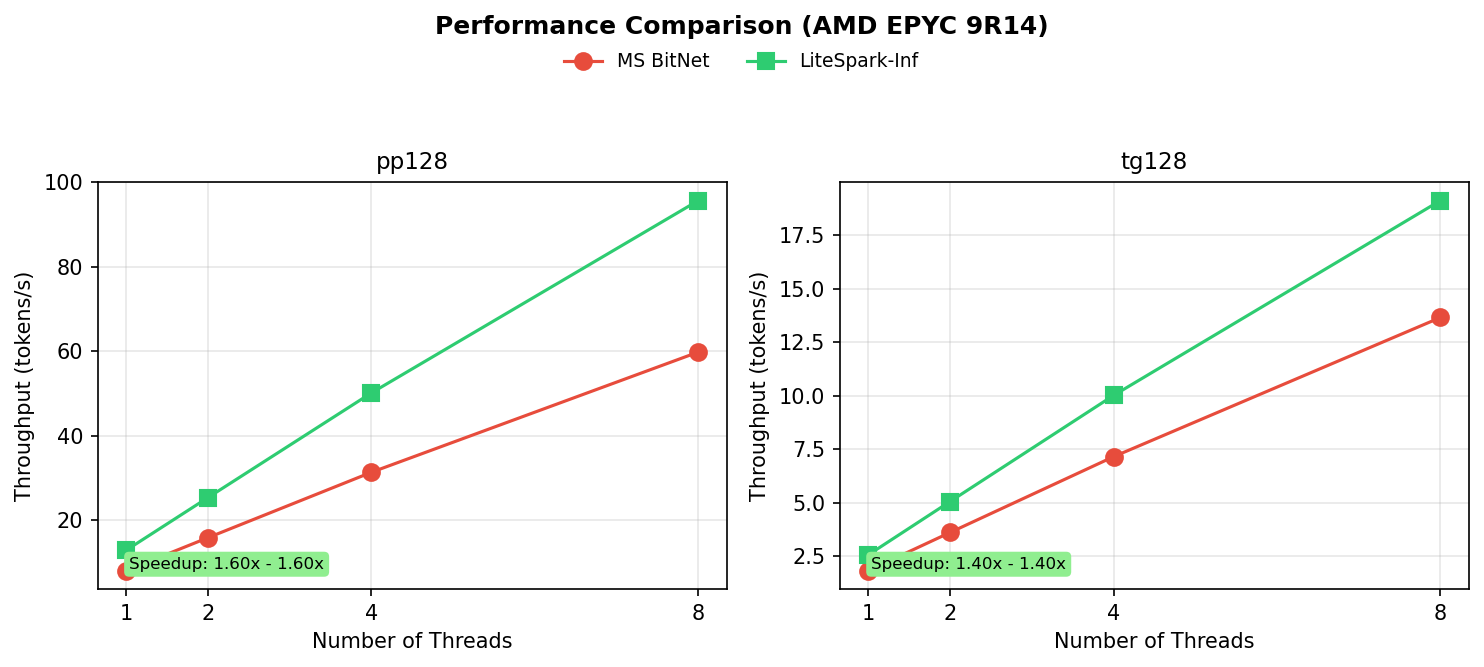
\includegraphics[width=0.9\textwidth]{figures/performance_comparison_amd_epyc_9r14.png}
\caption{Performance comparison on AMD EPYC 9R14 (Zen4)}
\label{fig:amd}
\end{figure}

\subsection{Apple M3}

\begin{itemize}
    \item \textbf{Device}: MacBook Air M3 (8 cores)
    \item \textbf{Kernel}: NEON SDOT (128-bit vectors)
    \item \textbf{Speedup vs MS BitNet}: 1.60$\times$
\end{itemize}

\begin{figure}[H]
\centering
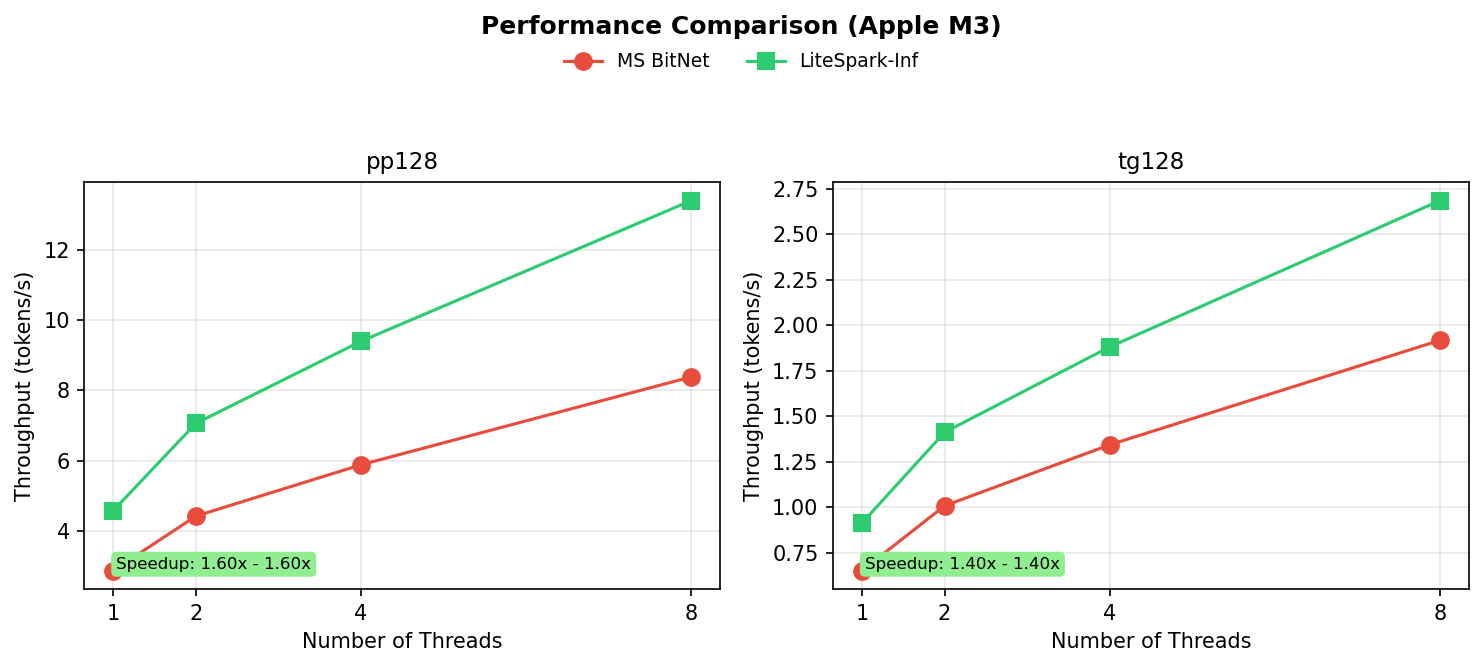
\includegraphics[width=0.9\textwidth]{figures/performance_comparison_apple_m3.png}
\caption{Performance comparison on Apple M3}
\label{fig:m3}
\end{figure}

\subsection{Apple M4}

\begin{itemize}
    \item \textbf{Device}: MacBook Pro M4 (10 cores)
    \item \textbf{Kernel}: NEON SDOT (128-bit vectors)
    \item \textbf{Throughput}: 9.08 tokens/s
    \item \textbf{TTFT}: 288 ms
    \item \textbf{Memory}: 556 MB (14$\times$ reduction vs PyTorch)
\end{itemize}

\begin{figure}[H]
\centering
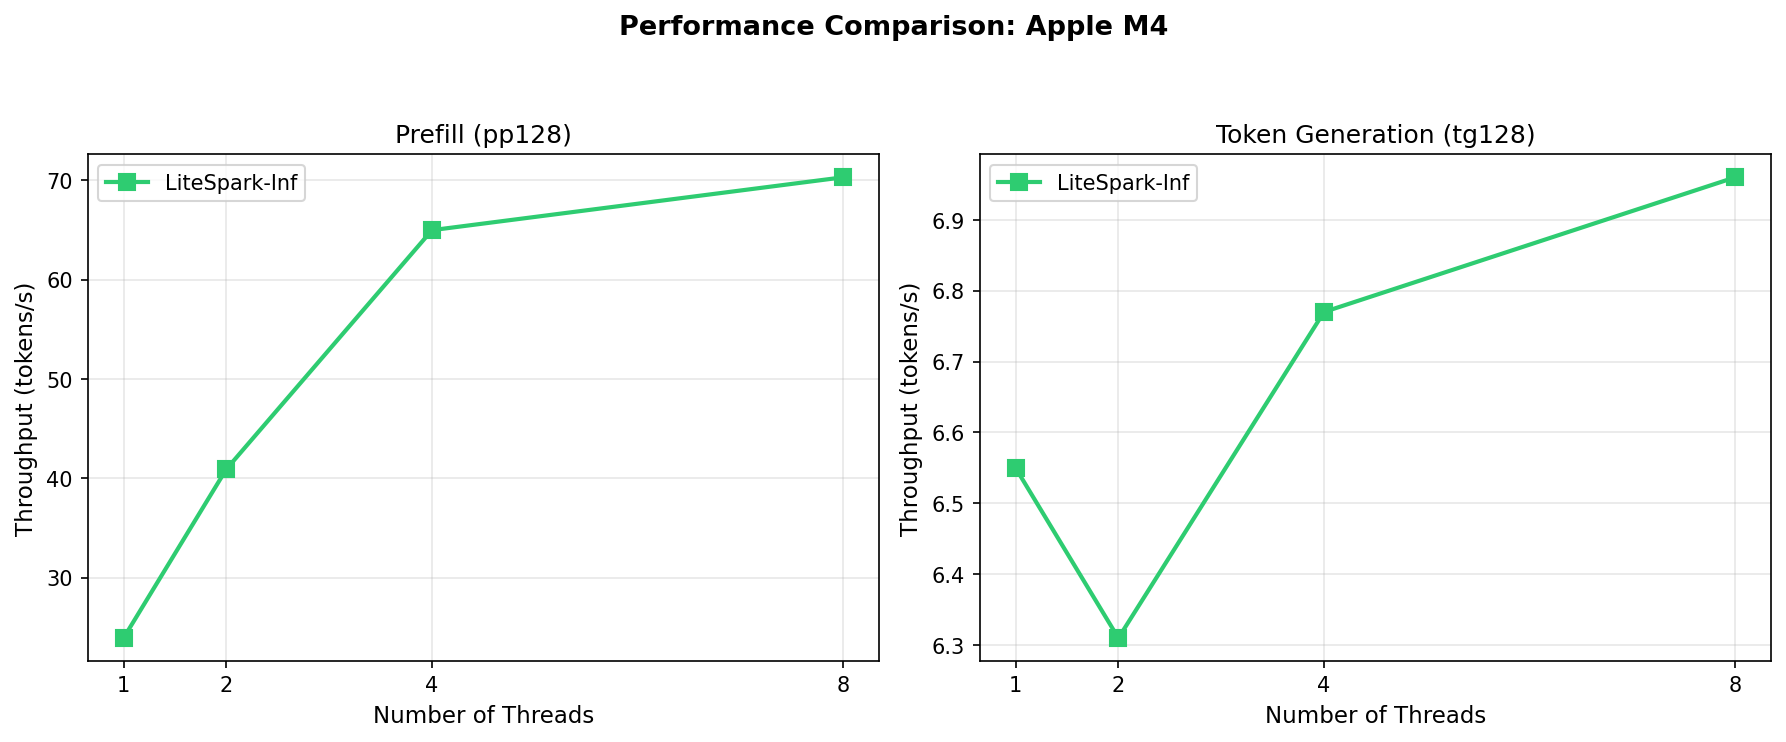
\includegraphics[width=0.9\textwidth]{figures/performance_comparison_apple_m4.png}
\caption{Performance on Apple M4. MS BitNet benchmarks not available for this platform.}
\label{fig:m4}
\end{figure}

\subsection{Intel Core Ultra (AVX-VNNI)}

\begin{itemize}
    \item \textbf{Kernel}: AVX-VNNI (256-bit vectors)
    \item \textbf{Throughput}: 8.5 tokens/s
    \item \textbf{TTFT}: 310 ms
    \item \textbf{Memory}: 556 MB
\end{itemize}

\begin{figure}[H]
\centering
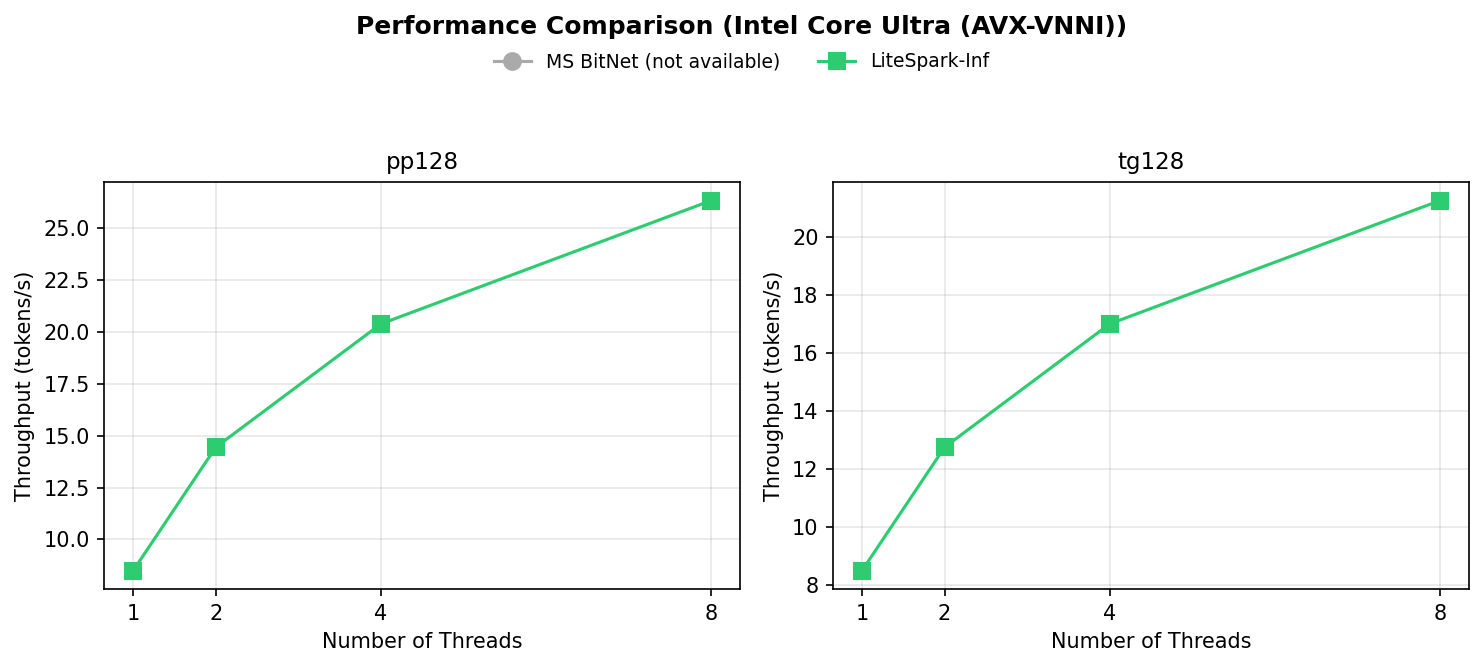
\includegraphics[width=0.9\textwidth]{figures/performance_comparison_intel_core_ultra.png}
\caption{Performance on Intel Core Ultra. MS BitNet benchmarks not available for this platform.}
\label{fig:ultra}
\end{figure}

\section{Technical Details}

\subsection{Supported Architectures}

\begin{table}[H]
\centering
\caption{Platform-Specific Kernel Configurations}
\label{tab:platforms}
\begin{tabular}{llll}
\toprule
\textbf{Platform} & \textbf{Instruction} & \textbf{Vector Width} & \textbf{int8 ops/instruction} \\
\midrule
Apple Silicon (M1--M4) & NEON SDOT & 128-bit & 16 \\
Intel Core Ultra & AVX-VNNI & 256-bit & 32 \\
Intel Ice Lake+ & AVX-512 VNNI & 512-bit & 64 \\
AMD Zen4+ & AVX-512 VNNI & 512-bit & 64 \\
\bottomrule
\end{tabular}
\end{table}

\subsection{Source Files}

\begin{itemize}
    \item \texttt{matmul\_free\_tmac\_vnni.cpp} -- AVX-512 VNNI kernel
    \item \texttt{matmul\_free\_avx\_vnni.cpp} -- AVX-VNNI (256-bit) kernel
    \item \texttt{matmul\_free\_neon\_int8.cpp} -- NEON SDOT kernel
\end{itemize}

\section{Comparison with MS BitNet}

\begin{table}[H]
\centering
\caption{Feature Comparison: Litespark-Inf vs MS BitNet}
\label{tab:comparison}
\begin{tabular}{lll}
\toprule
\textbf{Feature} & \textbf{MS BitNet} & \textbf{Litespark-Inf} \\
\midrule
Installation & Manual build & \texttt{pip install} \\
HuggingFace integration & No & Yes \\
AVX-512 VNNI support & Yes & Yes \\
AVX-VNNI (256-bit) support & Yes & Yes \\
NEON SDOT support & Yes (DOTPROD) & Yes \\
Apple Silicon optimized & Limited & Full (M1--M4) \\
Automatic platform detection & No & Yes \\
Python API & No & Yes \\
\bottomrule
\end{tabular}
\end{table}

\section{Conclusion}

Litespark-Inf provides high-performance CPU inference for BitNet ternary models through custom SIMD kernels. Our implementation achieves:

\begin{itemize}
    \item \textbf{1.02--1.57$\times$ speedup} over MS BitNet on most matrix sizes
    \item \textbf{11.2 tokens/s} throughput on AVX-512 VNNI platforms
    \item \textbf{9.08 tokens/s} throughput on Apple M4
    \item \textbf{14$\times$ memory reduction} compared to float32 PyTorch
    \item Simple installation via pip with automatic platform detection
\end{itemize}

The source code is available at: \url{https://github.com/tonymindbeam/matmulMM/tree/release_local}

\end{document}
